%pdflatex, utf8
\documentclass[unicode, 12pt, a4paper, oneside]{article}

\usepackage{anysize}
\marginsize{2cm}{1cm}{1cm}{1cm}

\usepackage[T2A]{fontenc}
\usepackage[utf8]{inputenc}
\usepackage[russian]{babel}

\usepackage{amsmath}
\usepackage{amsfonts}
\usepackage{amssymb}

\usepackage{color}
\usepackage{graphicx}
\graphicspath{{images/}}

\usepackage[hyphens]{url}
\usepackage[unicode]{hyperref}
\urlstyle{rm}

\usepackage{enumitem}
\setitemize{noitemsep,topsep=0pt,parsep=0pt,partopsep=0pt}
\setenumerate{noitemsep,topsep=0pt,parsep=0pt,partopsep=0pt}

\usepackage{textcomp}
\usepackage{cmap}

\newcounter{qcnt}
\newcommand{\quest}[1]{\par\refstepcounter{qcnt}\textbf{\arabic{qcnt}.\quad #1}}

\begin{document}

% Вопрос 1 ----------------------------------------------------------
\quest{Полупроводниковые приборы. Классификация. Область применения.}

Классификация П/П приборов:
\begin{itemize}
\item Полупроводниковые диоды
\item Полупроводниковые транзисторы
\item Полупроводниковые резисторы
\item Приборы с зарядной связью
\item Полупроводниковые лазеры
\item Оптоэлектронные приборы
\item Микросхемы
\end{itemize}

Принцип работы П/П приборов определяется электронно-дырочным переходом.
Полупроводниковым диодом называется прибор с двумя выводами и одним p-n переходом. Принцип работы полупроводникового диода основан на использовании односторонней проводимости, электрического пробоя и других свойств p-n перехода. Диоды различают по назначению, материалу, конструктивному исполнению, мощности и другим признакам.
Биполярным транзистором называется полупроводниковый прибор с двумя взаимодействующими p-n переходами. Биполярные транзисторы различаются по структуре. В зависимости от чередования областей различают биполярные транзисторы типа “p-n-p” и “n-p-n”. 
Полевые транзисторы. Полевым транзистором называется транзистор, в котором между двумя электродами образуется проводящий канал, по которому протекает ток. Управление этим током осуществляется электрическим полем, создаваемым третьим электродом. Электрод, с которого начинается движение носителей заряда, называется истоком, а электрод, к которому они движутся, стоком. Электрод, создающий управляющее электрическое поле, называется затвором. Различают два типа полевых транзисторов: с управляющим p-n переходом и с изолированным затвором (МДП-транзисторы). По типу электропроводности полевые транзисторы подразделяются на транзисторы с каналами "p" и "n" типов.
Полупроводниковые резисторы нашли широкое применение в электронных приборах. К ним относятся терморезисторы, магниторезисторы, варисторы, фоторезисторы. Принцип действия таких приборов основан на изменении свойств полупроводниковых материалов при воздействии на них температуры, магнитного и электрического полей, электромагнитного излучения.
Все п/п приборы делятся:
\begin{enumerate}
\item по технологии изготовления (из кремния, германия, арсенида галлия)
\item по принципу действия:
\begin{itemize}
\item диоды: выпрямительные, СВЧ, импульсные, смесительные, стабилитроны, стабисторы. Фотодиоды, светодиоды, тиристоры, денисторы
\item транзисторы: биполярные, полевые
\item резисторы: терморезисторы, магниторезисторы, варисторы, фоторезисторы
\end{itemize}
\end{enumerate}

% Вопрос 2 --------------------------------------------------------
\quest{Полупроводниковые диоды. Классификация. Область применения.}

Полупроводниковым диодом называется прибор с двумя выводами и одним p-n переходом. Принцип работы полупроводникового диода основан на использовании односторонней проводимости, электрического пробоя и других свойств p-n-перехода.
В зависимости от технологии изготовления различают точечные диоды, сплавные, микросплавные, эпитаксиальные и другие.
По функциональному назначению диоды делятся на выпрямительные, универсальные, импульсные, смесительные, СВЧ, стабилитроны, стабисторы, варикапы, динисторы, тиристоры, симисторы, фотодиоды, светодиоды и т.д.
По конструктивному исполнению диоды бывают плоскостные и точечные.
По используемому материалу - кремниевые, германиевые, арсенидгаллиевые. Диоды обладают односторонней проводимостью и служат: для выпрямления переменного тока, стабилизации тока и напряжения, формирования импульсов, для регулирования мощностей и т.д.
Выпрямительные диоды применяются для преобразования переменного тока в постоянный. Они делятся: на маломощные (до 0,3А), средней мощности (до 10А), мощные (более 1000А), низкочастотные (до 1кГц) и высокочастотные (до 100кГц).
Свойства выпрямительных диодов характеризуются вольтамперной характеристикой и параметрами, которые приводятся в справочной литературе.
Основные параметры диодов:
\begin{itemize}
\item средний выпрямленный ток Jср
\item прямое падение напряжения Uпр
\item обратный ток диода при заданной температуре Jобр
\item напряжение отсечки Uотс
\item мощность рассеивания Ррас
\item рабочая частота fр. и др.
\end{itemize}
\begin{figure}[htbp]
\centering
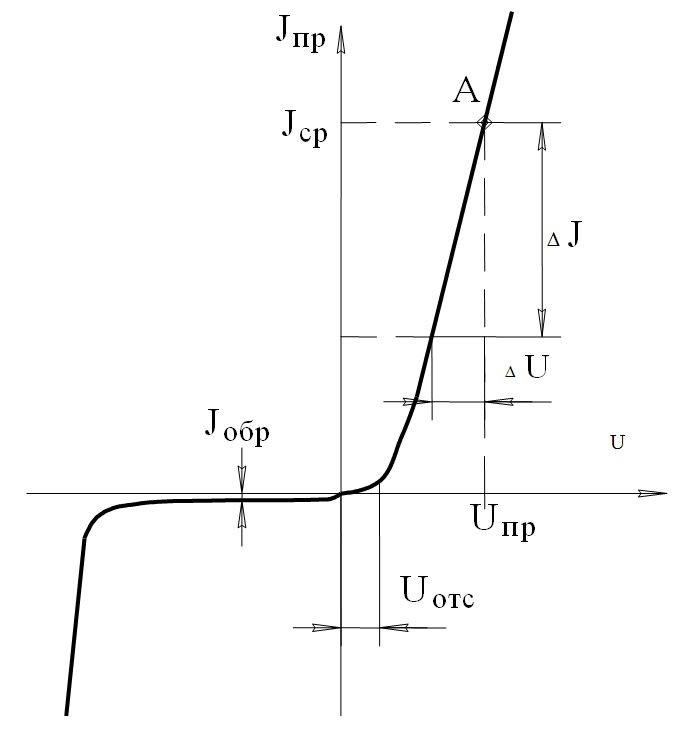
\includegraphics[width=0.8\textwidth]{2_VAC_of_diod.png}
\caption{ВАХ выпрямительного диода}
\label{fig:2_VAC_of_diod}
\end{figure}

Диоды обладают односторонней проводимостью и служат: для выпрямления переменного тока, стабилизации тока и напряжения, формирования импульсов, для регулирования мощностей и т.д.
Выпрямительные диоды применяются для преобразования переменного тока в постоянный. Они делятся: на маломощные (до 0,3А), средней мощности (до 10А), мощные (более 1000А), низкочастотные (до 1кГц) и высокочастотные (до 100кГц).
Свойства выпрямительных диодов характеризуются вольтамперной характеристикой и параметрами, которые приводятся в справочной литературе.
Основные параметры диодов средний выпрямленный ток Jср ,прямое падение напряжения Uпр ,обратный ток диода при заданной температуре Jобр., напряжение отсечки Uотс., мощность рассеивания Ррас., рабочая частота fр. и др.
Стабилитроны – это разновидность диодов, предназначенных для стабилизации напряжения. Вольт – амперная характеристика стабилитрона имеет вид. Рабочий участок характеристики АВ лежит в области электрического пробоя диода и характеризуется малым изменением напряжения Uст при значительных изменениях тока.
Стабисторы, как и стабилитроны, предназначены для стабилизации напряжения. Однако, в отличие от последних, рабочим участком у них является прямая ветвь вольт–амперной характеристики. Стабисторы работают при прямом напряжении и позволяют стабилизировать малые напряжения (0,35 - 1,9В).
Варикапы – это полупроводниковые диоды, емкость которых меняется при изменении обратного напряжения.


\quest{Полупроводниковые транзисторы. Классификация. Область применения.}
\quest{Полупроводниковые резисторы. Классификация. Область применения.}
\quest{Фотоэлектрические приборы. Классификация. Область применения.}
\quest{Аналоговые усилители. Классификация. Основные характеристики и параметры.}
\quest{Избирательные усилители. Усилители постоянного тока. Усилители мощности. Область применения.}
\quest{Операционные усилители. Классификация. Область применения. Балансировка ОУ.}
\quest{Стабилизаторы напряжения. Классификация. Параметры. Область применения.}
\quest{Логические операции. Схемная реализация.}
\quest{Цифровые устройства. Классификация. Комбинационные ЦУ. Дешифраторы, шифраторы, мультиплексоры, демультиплексоры.}
\quest{Комбинационные сумматоры.}
\quest{Триггера. Классификация. Область применения.}
\quest{Регистры и счетчики. Классификация. Схемы. Область применения.}
\quest{Цифро-аналоговые преобразователи. Назначение. Принцип работы. Матрица R-2R. Область применения.}
\quest{Аналого-цифровые преобразователи. Классификация. Область применения. Параллельные АЦП. АЦП поразрядного взвешивания.}
\quest{Интегрирующие АЦП. АЦП двойного интегрирования.}
\quest{Таймеры. Классификация. Область применения.}
\quest{Источники вторичного напряжения. Структурные схемы. Выпрямители и фильтры.}
\quest{Транзисторный усилительный каскад с общим эмиттером.}
\quest{Дискретные цифровые САР: математическое описание, Z передаточные функции.}
\quest{Анализ дискретных САР.}
\quest{Логарифмические частотные характеристики САР.}
\quest{Переходные функции и переходные характеристики САР. Реакция САР на произвольный входной сигнал.}
\quest{Типовые звенья САР и их частотные и временные характеристики.}
\quest{Устойчивость линейных САР: определение, теоремы Ляпунова, алгебраический критерий устойчивости Гурвица.}
\quest{Частотные критерии устойчивости линейных САР.}
\quest{Анализ качества линейных САР.}
\quest{Синтез корректирующих устройств линейных САР.}
\quest{Анализ нелинейных САР.}


\quest{Показатели качества ЭС.}

Показатели качества продукции – количественная характеристика определенного свойства продукции на определенном этапе жизненного цикла.

Показатели качества продукции делятся на следующие группы:
\begin{enumerate}
\item Назначения
\item Надежности
\item Технологичности
\item Эргономические
\item Эстетические
\item Стандартизация и унификация
\item Патентно-правовые
\item Экономические
\end{enumerate}

Единичный показатель качества --- показатель качества продукции, относящийся только к одному из её свойств. Комплексный показатель качества --- показатель качества продукции, относящийся к нескольким её свойствам.


\quest{Управление качеством ЭС.}

Управление качеством продукции базируется на статических методах контроля, зародилось в 30-е годы в связи с переходом к массовому производству изделий. В связи с этим стали применять выборочный контроль продукции с оценкой его результатов статистическим методом.

Контроль качества базируется на статистических методах и развиваясь циклически проходит через определенные этапы %(см. рис)

Для эффективного обеспечения контроля качества необходимо участие всех, без исключения , работников предприятия. Такой контроль качества называется Тотальным(TQC). Был придуман и внедрен впервые в Японии 60х годах.

Среди статистических методов можно выделить 7 наиболее эффективных и доступных:
\begin{enumerate}
\item Расслоение графики (полигон, гистограмма, кумулятивная кривая)
\item Расслоение общей изменчивости статистических данных с помощью дисперсионного анализа.
\item Диаграмма Парето
\item Причинно-следственная диаграмма
\item Диаграмма разброса (поле корреляции)
\item Контрольная карта
\item Контрольный лист
\end{enumerate}

\quest{Себестоимость и уровень качества ЭС.}
\quest{Корреляционная связь показателей ЭС.}
\quest{Метод расслаивания «ЧМ>>.}
\quest{Метод <<АВС-анализ>>.}
\quest{Виды статистического контроля ЭС.}
\quest{Количественные показатели надежности ЭС.}
\quest{Последовательная модель надежности ЭС.}
\quest{Параллельная модель надежности ЭС.}
\quest{Основные этапы автоматизации:  их характеристики и особенности}
\quest{Назначение, классификация и области применения роботов}
\quest{Манипуляционные роботы: типы, характеристики, применение}
\quest{Структура механизмов манипуляционных роботов и характеристики их геометрических свойств}
\quest{Приводы манипуляторов и роботов: классификация, особенности применения}
\quest{Конструкции схватов промышленных роботов, особенности применения}
\quest{Проектирование  архитектуры интегрированной компьютерной системы управления }
\quest{Описание технологического процесса как объекта автоматизированного управления }
\quest{Описание производственного процесса как объекта автоматизированного управления: реализация АРМ различных уровней}
\quest{Выбор датчиков технологического процесса: типы измерительных устройств,  подключение.}
\quest{Теорема Котельникова (теорема отсчетов). Квазидетерминированные сигналы.}
\quest{Преобразование измерительных сигналов. Виды модуляций.}
\quest{Цифровые частотомеры.}
\quest{Цифровые фазометры.}
\quest{Цифровые вольтметры временного преобразования.}
\quest{Микропроцессорные цифровые измерительные преобразователи.}
\quest{Резистивные датчики (реостатные, пьезорезистивные).}
\quest{Электромагнитные датчики (индуктивные, трансформаторные, магнитоупругие).}
\quest{Пьезоэлектрические датчики.}
\quest{Тепловые датчики (термопары, термометры сопротивления).}
\quest{Организация и этапы разработки конструкторских документов.}
\quest{Виды КД.}
\quest{Стандартизация и БНК.}
\quest{Виды и типы схем, обозначения по ЕСКД.}
\quest{Методы компоновки конструкции ЭВС.}
\quest{Климатические зоны и категории исполнения.}
\quest{Способы защиты ЭВС от влаги.}
\quest{Защита ЭВС от механических воздействий.}
\quest{Способы обеспечения теплового режима ЭВС.}
\quest{Электромагнитные воздействия. Виды экранов.}
\quest{Виды линий связи.}
\quest{Особенности конструирования бортовых ЭВС.}
\quest{Особенности конструкций персональных ЭВМ.}
\quest{Унификация. Разновидности стандартизации.}
\quest{Требования к трассировке ПП и электрическим соединениям.}
\quest{Электромонтажные провода. Припои и флюсы.}
\quest{Волоконно-оптические линии связи (ВОЛС). Примеры использования.}
\quest{Эргономические требования к пультам, органам управления и сигнализации.}
\quest{Эргономика конструирования лицевой панели прибора.}
\quest{Защита ЭС от воздействий радиации.}
\quest{Производственный и технологический процесс и их составляющие.}
\quest{Исходные данные для разработки технологических процессов. Основные этапы разработки единичного технологического процесса.}
\quest{Требования к оформлению технологической документации. Примеры записи технологических операций.}
\quest{Основные методы изготовления печатных плат и их особенности.}
\quest{Конструктивно-технологические разновидности радиоэлектронных узлов и их сопоставительный анализ.}
\quest{Основные технологические операции при изготовлении радиоэлектронных узлов с монтажом на поверхность.}
\quest{Нанесение паяльной пасты и клея и используемое при этом оборудование.}
\quest{Принципы организации работы сборочных автоматов.}
\quest{Особенности выполнения пайки при изготовлении электронных модулей (пайка оплавлением, волной припоя, селективная пайка).}
\quest{Особенности выполнения ремонтных работ: демонтаж и монтаж компонентов.}
\quest{Материалы, используемые в технологии монтажа на поверхность.}
\quest{Виды соединительных операций при сборке.}
\quest{Соединение сваркой: разновидности, области применения.}
\quest{Соединение пайкой: разновидности, области применения, примеряя выполнения паяных соединений.}
\quest{Разработка схемы сборки изделий.}
\quest{Нормирование затрат времени при проектировании технологических процессов (штучное и подготовительно-заключительное время, определение такта и ритма выпуска изделий).}
\quest{Изготовление деталей ЭС методом литья.}
\quest{Разделительные и формообразующие операции холодной штамповки.}
\quest{Общая характеристика методов формообразования материалов и деталей при производстве ЭС.}
\quest{Изготовление электронных модулей по технологии внутреннего монтажа.}


\quest{Приведите структуру контроллера (микроЭВМ) с раздельными шинами адрес/данные и следующим составом: ХХ кб, ПЗУ – ХХ кб, индикация – 1, порты ввода/вывода – Х клавиатура – 1. Распределите адресное пространство для контроллера. Приведите таблицу распределения адресов.}

\begin{center}
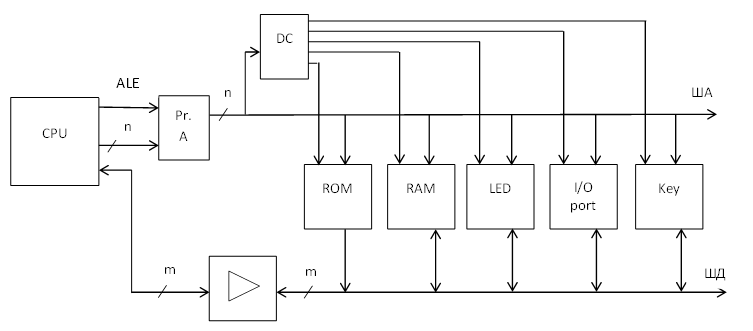
\includegraphics[width=0.8\textwidth]{101_struct.png}\\
\end{center}

Допустим шина адреса процессора включает 16 бит, а шина данных – 8 бит, тогда максимальный объем адресуемой памяти составит 64 Кбайт. Предположим что для ОЗУ необходимо выделить 32 Кбайта, ПЗУ – 8 Кбайт, индикация – 256 байт, порт ввода/вывода – 256 байт, клавиатура – 256 байт. При делении адресного пространства между блоками необходимо соблюдать, чтобы начальный адрес каждого блока начинался с нулей, а старший заканчивался на “F”.
\begin{center}

\begin{tabular}{|c|c|c|}
\hline 4000h - AFFFh & ОЗУ &  32 Кбайт  \\ 
\hline 3200h - 32FFh & порт ввода/вывода &  256 байт  \\ 
\hline 3100h - 31FFh & клавиатура & 256 байт  \\  
\hline 3000h - 30FFh & индикация & 256 байт  \\  
\hline 1000h - 2FFFh & ПЗУ &  8 Кбайт  \\ 
\hline 0000h - 0FFFh & регистры процессора & 4 Кбайт  \\ 
\hline 
\end{tabular} 

\end{center}
\quest{Укажите место на структурной схеме ЭВМ различных интерфейсов. Как объединять ЭВМ в  систему? Какие условия следует выполнить при  передаче данных? Обоснуйте.}
\quest{Расставьте по убыванию значимости параметры ЭВМ по критерию производительности. Охарактеризуйте эти параметры.}
\quest{Преобразуйте десятичное число в различные форматы хранения. В какой форме хранятся в памяти ЭВМ символы. Приведите два примера.}
\quest{Сопоставьте принципы печати лазерного и струйного принтеров, опишите и сравните их.}
\quest{Приведите две схемы подключения клавиатуры к портам ввода-вывода. Приведите алгоритм опроса пассивной матричной клавиатуры.}
\quest{Выберите способ обмена данными между процессором и внешним устройством. Обоснуйте выбор. Напишите процедуру ввода или вывода данных в память ЭВМ в мнемонике команд (уровень ассемблера).}
\quest{Приведите основные архитектурные варианта построения операционных систем. Поясните понятие <<виртуальная машина>>.}
\quest{Спроектировать устройство управления программного типа. Число микрокоманд в цикле – не более 7. Привести примеры циклов: выборка команды, чтение памяти и запись в память. Чем определяется период следования тактового сигнала.}
\quest{Спроектировать устройство микропрограммного управления автономного типа. Источник управляющих кодов – счетчик микрокоманд, число состояний счетчика – 32. Разрядность регистра микрокоманд – 24.}
\quest{Привести примеры процедур с различными способами адресации для пересылки содержимого ячейки памяти команд в ячейку памяти данных в мнемонике команд, адресация в пределах одной страницы (64 кб). Пояснить необходимость модификации адресов для доступа к данным и возможные их способы.}
\quest{Прерывания как способ изменения адреса в управляющей команде. Привести пример системы прерывания. Описать процедуру опознавания запроса на прерывание с маскированием.}
\quest{Системы памяти ЭВМ. Назначение каждого типа элементов памяти и место его в иерархии. Что дает для характеристик ЭВМ каждый тип элементов памяти.}
\quest{Память программ. Виды носителей. Жесткие диски и их твердотельные аналоги.}
\quest{Компиляторы. Назначение компиляторов, их виды. Последовательность процедуры компиляции.}
\quest{Контроль информации при последовательной передаче двоичного кода. Методы контроля. Контроль передачи информации при обмене словами (байтами). Методы.}
\quest{Приведите основные структуры объединения процессоров в многопроцессорных системах. В чем суть ограничений архитектуры Фон-Неймана.}
\quest{Сравните структуры двух МПК, имеющих организацию SMP и MPP. Приведите их структурные схемы.}
\quest{Сравните характеристики двух последовательных интерфейсов RS-232С и USB. Приведите  структурную организацию интерфейсов и формат передаваемых данных.}
\quest{Какие принципы программного управления характерны для командного и микро-командного способов управления. В чем сходство и различие этих способов. Покажите на примере структурной схемы устройств управления.}
\quest{Основные понятия процесса проектирования систем управления. Цель процесса проектирования.}
\quest{Системный подход к проектированию.}
\quest{Структура процесса автоматизированного проектирования.}
\quest{Основные типы автоматизированных систем, разновидности САПР.}
\quest{Стадии проектирования автоматизированных систем и аспекты их описания.}
\quest{Особенности проектирования САПР.}
\quest{Понятие о CALS-технологиях.}
\quest{Открытые системы.}
\quest{Техническое обеспечение систем автоматизированного проектирования.}
\quest{Типы сетей, методы доступа в сетях, протоколы и стеки протоколов в вычислительных сетях.}
\quest{САПР систем управления.}
\quest{Автоматизация управления предприятием, логистические системы.}
\quest{АСУТП, автоматизированные системы делопроизводства.}
\quest{Математическое обеспечение анализа проектных решений.}
\quest{Компоненты математического обеспечения, структура вычислительного процесса анализа.}
\quest{Математическое обеспечение анализа на макроуровне.}
\quest{Математическое обеспечение анализа на микроуровне.}
\quest{Математическое обеспечение анализа на функционально-логическом уровне.}
\quest{Математическое обеспечение анализа на системном уровне.}
\quest{Математическое обеспечение подсистем машинной графики и геометрического моделирования.}
\quest{Схемы мультивибратора на транзисторах и ОУ.}
\quest{Схема одновибратора на транзисторах.}
\quest{Масштабный усилитель на ОУ с К=+10.}
\quest{Повторитель на ОУ.}
\quest{Двухтактный трансформаторный усилитель мощности, работающий в режиме АВ.}
\quest{Избирательные усилители LC и RC.}
\quest{Схема стабилизатора напряжения на 10 В, 2 А на ИС К142.}
\quest{Схема стабилизатора напряжения на 12 В, 1 А на ИС К142.}
\quest{Схема ключевого стабилизатора напряжения.}
\quest{Генератор гармонических колебаний на транзисторах.}


\quest{Системы хранения данных. Назначение. Три основные структуры систем хранения данных.}

С ростом производительности ЭВМ и увеличением объемов хранимой информации возникает необходимость в специальных внешних устройствах для хранения данных. ВЗУ большого объема обычно строятся на основе ленточных накопителей, которые обладают большим временем доступа и быстрым старением. Возникает задача хранения больших объемов данных с быстрым временем доступа.

Причинами появления СХД считают следующие: децентрализация хранения информации (организациям со временем приходится задействовать оборудование филиалов для хранения информации), низкий уровень защиты данных, низкая степень конфиденциальности передаваемых данных, требования к масштабируемости (неизвестно какие объемы информации потребуется хранить через несколько лет). Возникает необходимость в некой автоматизированной системе, которая хранила бы данные.

В простейшем случае структуру такой системы можно представить в следующем виде: \mbox{SCSI --- RAID-контроллер --- HDD (несколько)}.

К SCSI подключается RAID-контроллер с буферным каналом ввода/вывода и кэш-памятью достаточно большого объема. Задача RAID-контроллера обеспечить формирование RAID-массива: присваивание файлам своих адресов, причем связь контроллера с HDD осуществляется по параллельным линиям с электрическими или оптическими сигналами.

За счет кэш-памяти RAID-контроллер обеспечивает высокую скорость доступа к данным, при этом задача буферного блока скомпоновать общий файл при нескольких запросах. Кроме того, в буферном блоке производится контроль информации, при необходимости с восстановлением.

Такие СХД подключаются к типовым интерфейсам, прежде всего к SCSI (до 640 Мб/с). Помимо него часто используется Fibre Channel --- интерфейс с оптическими линиями связи способный обеспечивать до 4 Гб/с.

\textbf{Структура СХД}. Для подключения внешних дисков требуется внешний контроллер с высоким быстродействием, чтобы обеспечить приемлемую скорость передачи массива. Передача идет файлам не непрерывно, с попеременными чтением и записью, поэтому в структуру СХД должны входить следующие блоки:

\begin{center}
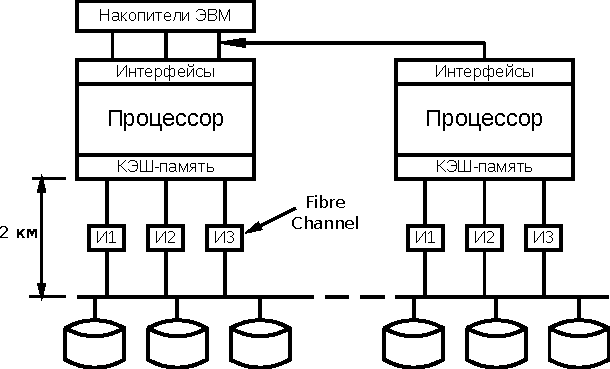
\includegraphics[width=0.6\textwidth]{./images/151_struct.pdf}
\end{center}

\textbf{Организация СХД}. В зависимости от объемов хранимой информации, сложности системы и требований к надежности можно выделить три основные структуры СХД:

\textbf{Прямое включение <<DAS>>}. Сервер сети и сервер СХД разделены. Имеется толь одна линия доступа к СХД, что снижает надежность и скорость доступа к данным.

\begin{center}
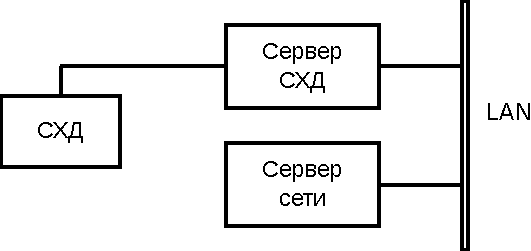
\includegraphics[width=0.4\textwidth]{151_das.pdf}
\end{center}

\textbf{Прямое подключение в сеть <<NAS>>}. СХД является абонентом сети, обеспечивающим файловый доступ, и должна иметь соответствующее сетевое оборудование. У каждой стойки может быть свое особенное ПО.

\begin{center}
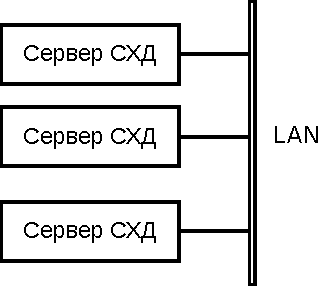
\includegraphics[width=0.25\textwidth]{151_nas.pdf}
\end{center}

\textbf{Сетевое подключение <<SAN>>}. Имеется возможность переключения каналов передачи информации. СХД подключается сразу к 2 каналам и, если один из них загружен, то используется второй. Система централизованная, но сложная и дорогая.

\begin{center}
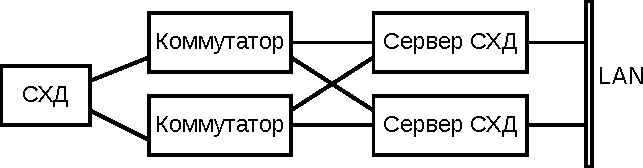
\includegraphics[width=0.6\textwidth]{151_san.pdf}
\end{center}


\quest{Основные понятия информационно-вычислительных систем, классификация по критерию потоков информации.}
\quest{Совмещение операций и многопрограммная работа. Режим работы в реальном времени.}
\quest{Типы структур многопроцессорных ВС. Параллельные ЭВМ, классификация. Три архитектурных класса машин.}
\quest{Принципы ввода-вывода информации в ПЭВМ. Роль и структура контроллера ввода информации.}


\quest{Программная реализация ввода чисел с клавиатуры. Привести алгоритм ввода двухразрядного числа с клавиатуры для его суммирования с другими числами.}

Принцип действия универсальной клавиатуры основан на формировании клавиатурного прерывания при нажатии клавиши. Клавиатурное прерывание является внешним и имеет свой вектор. Получив запрос на прерывание, процессор завершает текущую операцию, читает порт клавиатуры (60h) и переписывает код клавиши в буфер клавиатуры, расположенный в области данных BIOS в ОЗУ.
Чтение из буфера можно произвести с помощью стандартных подпрограмм BIOS (int 16h) и DOS (int 21h). В зависимости от подпрограммы процессор читает из буфера один символ (например: mov ah,00h; int 16h) или последовательность символов (например: mov ah,3fh; int 21h).

Т.к. использование таких функций позволяет получить коды символов, то для возможности работы с введенным числом необходимо преобразовать коды символов в двоичный код.  Алгоритм ввода двухразрядного числа для последующей работы с ним ([30h, 39h] — диапазон ASCII-кодов цифр):

Ожидать нажатия клавиши; Сохранить в регистре код нажатой клавиши; Проверить вхождение кода в диапазон [30h, 39h] (если не входит, вывести ошибку, повторить ввод); Отнять от кода 30h; Умножить код на 10; Переслать код в ячейку памяти; Ожидать нажатия клавиши; Сохранить в регистре код нажатой клавиши;  Проверить вхождение кода в диапазон [30h, 39h] (если не входит, вывести ошибку, повторить ввод); Отнять от кода 30h; Прибавить код к содержимому ячейки памяти;


\quest{Вывод информации на дисплей. Принципы отображения информации на экране дисплея. LCD- дисплеи.}
\quest{Процедура вывода символьной информации на дискретные индикаторы.}
\quest{Загрузчики. Процедура загрузки. Статические и динамические загрузки.}


\quest{Управление реальной памятью. Виртуальная память. Таблица соответствия адресов.}

В многопрограммном режиме работы возникает задача размещения загружаемых программ в ОЗУ.  Участки памяти, куда загружаются программы, определяются с помощью программы управления памятью — диспетчера памяти. В зависимости от сложности задачи выделяют несколько стратегий управления памятью:

\textbf{Статическое деление} --- разделение памяти на участки фиксированного объема, обычно применяется в простейших случаях (2-3 программы). Если процессов много, часть из них должна ожидать своей очереди для размещения в памяти, пока не завершатся предыдущие загруженные программы. Загрузка программы возможна только в том случае, если объем раздела в памяти больше объема программы, следовательно с такой системой загрузки всегда остается неиспользуемое свободное место в памяти, что снижает эффективность ее использования.

\textbf{По запросу} --- деление памяти на фрагменты переменной длины. Процессы стоящие в очереди получают необходимый для загрузки объем памяти, следовательно память используется эффективнее. Когда один или несколько процессов завершатся, в освободившуюся область памяти загружаются новые процессы из очереди, которые однако имеют другой размер, поэтому в занимаемой памяти образуются <<дыры>>. Чтобы исправить эту проблему производится \textbf{дефрагментация} --- сдвиг одного из массивов к окончанию другого. При этом возникает задача нахождения в кодах абсолютных ссылок и изменения их, для их нахождения команды переходов по абсолютным адресам могут быть отмечены специальным битом (технически это не предусмотрено в системе команд) либо при компиляции в конец файла могут быть записаны адреса таких команд. Для выполнения дефрагментации требуется специальная программа для пересылки массивов.

Другая проблема возникает, когда работающий процесс затребовал дополнительную память, поэтому массив новых данных формируется в другом сегменте памяти. В таком случае программа управления памятью работает как редактор связей: делает ссылку в текущих кодах на новое адресное пространство.

Загрузку программ в память выполняет загрузчик, который выполняет пересылку по необходимым адресам. Загрузка в память выполняется по параграфам (младшая тетрада адреса загрузки равна нулю). Загрузка может производиться в статическом (сначала загружаются все задачи, затем выполняются), либо в динамическом (в промежутках между работой загружаются другие задачи) режимах.

Основная память ВС ограничена, в то же время используя ВЗУ можно попеременно по одним и тем же адресам в основной памяти загружать коды из внешней памяти и работать с ними. Такую организацию памяти называют виртуальной. Основная проблема при таком алгоритме работы — связывание конкретной задачи с адресами в ВЗУ. Кроме того, при работе с файлам может возникнуть необходимость сохранения их в ВЗУ, для этого используется таблица соответствия адресов.

\begin{center} % Можно заюзать окружение figure, но тут оно не очень и нужно.
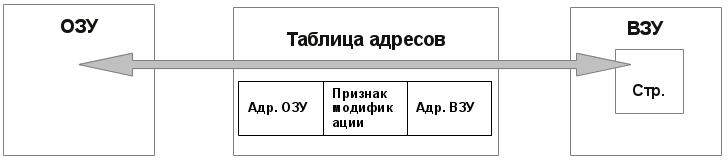
\includegraphics[width=0.8\textwidth]{virt_mem.png}\\
Таблица адресов содержит: адрес в ОЗУ, адрес в ВЗУ, признак модификации.
\end{center}

\end{document}
